% This file was created by tikzplotlib v0.9.8.
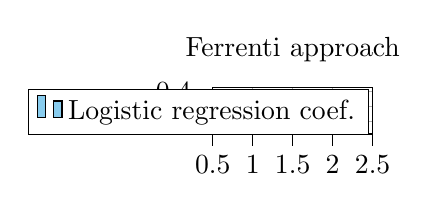
\begin{tikzpicture}

\definecolor{color0}{rgb}{0.533333333333333,0.8,0.933333333333333}

\begin{axis}[
height=0.8533462847654628in,
tick align=outside,
tick pos=left,
title={Ferrenti approach},
width=1.4222438079424382in,
x grid style={white!69.0196078431373!black},
xmajorgrids,
xmin=0.5, xmax=2.5,
xtick style={color=black},
y grid style={white!69.0196078431373!black},
ymajorgrids,
ymin=-0.173064253300487, ymax=0.454074936965614,
ytick style={color=black}
]
\draw[draw=none,fill=color0] (axis cs:0.6,0) rectangle (axis cs:1.4,-0.123064253300487);
\addlegendimage{ybar,ybar legend,draw=none,fill=color0};
\addlegendentry{Logistic regression coef.}

\draw[draw=none,fill=color0] (axis cs:1.6,0) rectangle (axis cs:2.4,0.254074936965614);
\path [draw=color0, semithick]
(axis cs:1,-0.229417488366355)
--(axis cs:1,-0.0167110182346182);

\path [draw=color0, semithick]
(axis cs:2,0.23592009450898)
--(axis cs:2,0.272229779422249);

\addplot [semithick, color0, mark=-, mark size=4, mark options={solid}, only marks]
table {%
1 -0.229417488366355
2 0.23592009450898
};
\addplot [semithick, color0, mark=-, mark size=4, mark options={solid}, only marks]
table {%
1 -0.0167110182346182
2 0.272229779422249
};
\end{axis}

\end{tikzpicture}
